
%% modelo.tex
%% V1.0
%% 03/05/2009
%% Hugo Vieira Neto
%%
%% Modelo de artigo de conferência IEEE para LaTeX
%% Requer os arquivos IEEEtran.cls, IEEEtran.bst e IEEEabrv.bib

% *** PREÂMBULO ***
\documentclass[conference,peerreview]{IEEEtran}
% Na versão final do artigo, a opção peerreview deve ser removida para
% que as informações sobre os autores fiquem aparentes após o título.

% Pacotes para a utilização da língua portuguesa.
\usepackage[brazil]{babel}
\usepackage[utf8]{inputenc}
% As linhas acima devem ser comentadas se o artigo for escrito em inglês.

% Pacotes para o uso de equações e símbolos matemáticos.
\usepackage[cmex10]{amsmath}
\usepackage{amsfonts,amssymb}

% Pacotes para o uso de tabelas, gráficos e subfiguras.
\usepackage{array}
\usepackage{graphicx}
\usepackage[caption=false,font=footnotesize]{subfig}

% Pacote para a formatação ordenada automática de múltiplas citações.
\usepackage{cite}

% Pacote para a formatação adequada de URL.
\usepackage{url}

% Falhas de separação em sílabas devem ser listadas aqui
\hyphenation{}


% *** CORPO DO TEXTO ***
\begin{document}

% Título do artigo
\title{Aprendizado de máquinas e Espectroscopia Raman para identificação de fungos}
% Quebras de linha \\ podem ser inseridas para melhor formatação de títulos
% longos.


% Nome e afiliação do autor
\author{
	\IEEEauthorblockN{Daniel Silva Costa}
	\IEEEauthorblockA{
		CPGEI / UTFPR\\
		Avenida Sete de Setembro, 3165\\
		Curitiba-PR - CEP 80.230-910\\
		E-mail: eng.daniels.costa@gmail.com\\
		\url{https://github.com/danielscosta}
	} % \IEEEauthorblockA
} % \author
% Para múltiplos autores e afiliações, consultar exemplos no arquivo
% bare_conf.tex


% Formatação do título e autoria do artigo. Em artigos com a opção peerreview,
% a autoria é ocultada e as páginas são numeradas.
\ifCLASSOPTIONpeerreview
	\setcounter{page}{1}
	\IEEEpeerreviewmaketitle
\else
	\maketitle
\fi


% Resumo do artigo
\begin{abstract}
A identificação da espécie de um fungo causador de doenças é determinante na escolha do tratamento mais adequado. Contudo tal tarefa pode ser desafiadora dadas as semelhanças entre as espécies de mesmo gênero. Para tanto, pode ser utilizado o sequenciamento genético, entretanto, é uma técnica de elevado custo e requer equipamentos que não estão facilmente disponíveis. Este trabalho apresenta uma proposta de projeto para analisar dados do espectro Raman de alguns fungos através de técnicas de aprendizado de máquinas, de forma que, consiga-se identificar quais dados são relevantes para diferenciação e identificação de uma espécie específica dentre as analisadas, além de criar uma rede neural artificial treinada com esse propósito. A relevância desta proposição está na elaboração de um método mais barato e simples para identificar espécies de fungos com gêneros iguais. 
\end{abstract}

\section{Introdução}
O Reino Fungi é composto pelas mais variadas formas de seres, desde micro-organismos até cogumelos. Contudo, quando deseja-se diferenciar espécies de mesmo gênero (táxon da classificação biológica) isto torna-se uma tarefa árdua, pois tais diferenças só são perceptíveis nas estruturas celulares destes seres, como pode ser verificado na figura \ref{fungus_dif}.

\begin{figure}[ht]
\centering
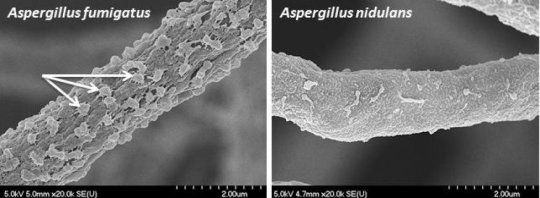
\includegraphics[width=8.5cm]{fungus_dif}
\caption{Diferença nas estruturas celulares das espécies fungos fumigatus e nidulans ambos do gênero Aspergillus. Fonte: \cite{Lee2015}}
\label{fungus_dif}
\end{figure}

Realizar o sequênciamento genético de uma amostra de células de um fungo é a forma mais assertiva de determinar a qual espécie o mesmo pertence. Mas, é um método com alto custo e requer um sequenciador genético a disposição. Por isto este trabalho propõe a utilização de dados de Espectroscopia Raman das células dos fungos para criar uma modelo de aprendizagem de máquina capaz de identificar a espécie de um fungo.

A Espectroscopia Raman é uma técnica que necessita de equipamentos simples para sua execução: microscópio ótico comum, laser de excitação, monocromador e um detector sensível (Figura \ref{esquema_experimento}). E, apesar de simples, ela pode gerar informação de qualidade sobre a composição da amostra que se analisa. Mas interpretar seus resultados é uma tarefa complexa, por isso, utilizar técnicas de aprendizado de máquina podem ajudar a identificar os padrões nos dados do espectro Raman.

\begin{figure}[ht]
\centering
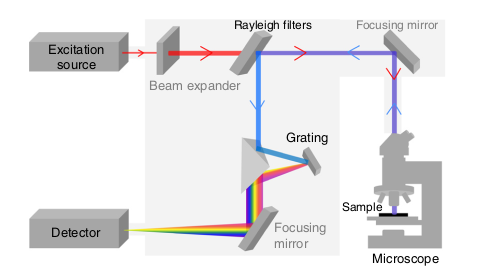
\includegraphics[width=8cm]{esquema_experimento}
\caption{Esquema técnico das Espectroscopia Raman. Fonte: \cite{Butler2016}}
\label{esquema_experimento}
\end{figure}

Nas próximas seções serão detalhadas a significância do sinal da Espectroscopia Raman para o caso de estudo, PCA(Principal Component Analysis) e Redes Neurais Artificiais e será realizada uma discussão do porquê estas técnicas podem trazer um valor significante à matéria de estudo, além de apresentar os resultados esperados ao fim desta pesquisa.

\section{Aspectos teóricos}

Espectroscopia Raman é uma técnica que foi inspirada em um fenômeno observado experimentalmente por Chandrasekhara Venkata Raman. Tal fenômeno consiste no espalhamento da luz em diferentes frequências ao incidir um laser sobre um material. Essas frequências luminosas se espalham devido a vibração entre as moléculas que foram excitadas pela luz incidida. A Figura \ref{incidencia_luminosa_exemplo} apresenta o esquemático do fenômeno descrito.

\begin{figure}[ht]
\centering
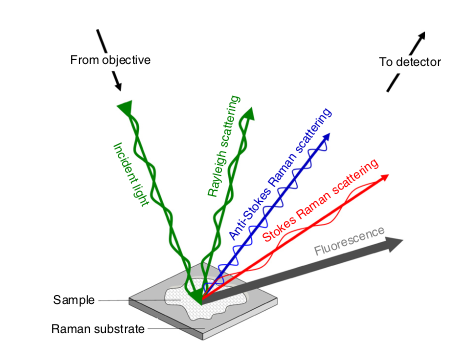
\includegraphics[width=6.5cm]{incidencia_luminosa_exemplo}
\caption{Esquema do efeito Raman. Fonte: \cite{Butler2016}}
\label{incidencia_luminosa_exemplo}
\end{figure}

O conjunto das frequências luminosas espalhadas compõe uma assinatura que reflete a composição do material analisado, cada tipo de estrutura molecular vibrará em uma intensidade, por isso, espalhará a luz em uma frequência diferente. Alguns exemplos de assinaturas geradas podem ser verificados na figura \ref{assinatura_raman_exemplo}.

\begin{figure}[ht]
\centering
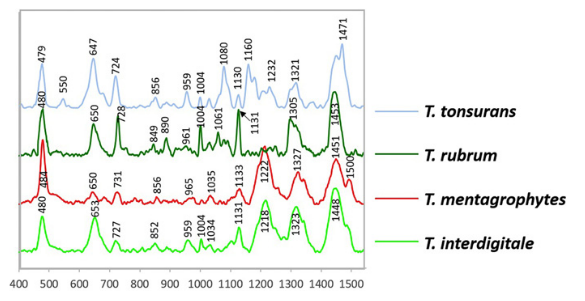
\includegraphics[width=9.5cm]{assinatura_raman_exemplo}
\caption{Exemplo de assinaturas obtidas atravês da Espectroscopia Raman. Cada cor reflete uma medição para espécies diferentes de fungos do gênero Trichophyton. Fonte: \cite{Pankin2018}}
\label{assinatura_raman_exemplo}
\end{figure}

Quando se realiza uma medição do espectro Raman, é preparada uma solução aquosa adicionando uma pequena quantidade do material que se deseja analisar e se adiciona um substrato à amostra (geralmente metais nobres) que por sua vez servirão como amplificadores da intensidade luminosa espalhada. A escolha do substrato é parte crucial na obtenção dos dados do espectro Raman conforme \cite{Seifert2016}, pois ruídos podem ser gerados pelo substrato escolhido distorcendo os resultados.

Uma vez obtidos os dados referentes ao espectro Raman é comum utilizar ferramental matemático para extrair da assinatura obtida ruídos advindos da fluorescência da composição material da amostra. Tal aspecto pode, por sua vez, mascarar a informação relevante do sinal que em geral é caracterizada por picos.

O PCA é uma das ferramentas utilizadas para eliminar os ruídos do espectro Raman. Este método matemático é capaz de identificar em um espaço amostral de n dimensões quais destas carregam informação realmente relevantes para análise. Contudo, a eficiência deste método está no agrupamento de informação em poucas dimensões. Caso exista grande variação entre várias das componentes das amostras, ao considerar apenas as de maior variância, muita informação relevante pode ser perdida comprometendo a análise que se deseja realizar \cite{Brereton2017}. Por isso plotar as relações entre as componentes de maior variância pode ter grande valor analítico, pois se a significância não estiver sendo perdida padrões de agrupamento poderão ser visualizados. A Figura \ref{pca_exemplo} demonstra o surgimento destes padrões de agrupamento na análise de amostras de pólen realizadas em \cite{Seifert2016}.

\begin{figure}[ht]
\centering
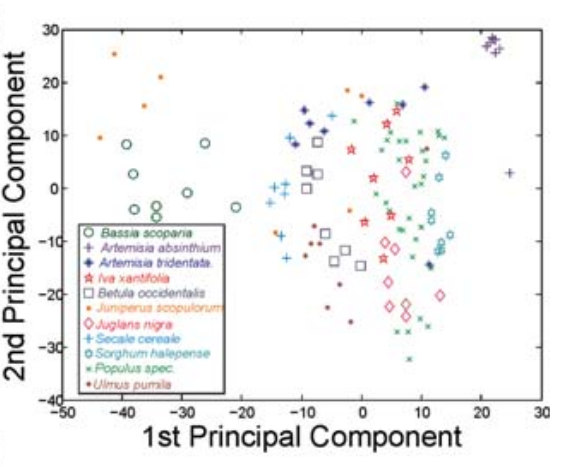
\includegraphics[width=6.5cm]{pca_exemplo}
\caption{Análise das principais componentes do espectro Raman de amostras de pólen. Fonte: \cite{Seifert2016}}
\label{pca_exemplo}
\end{figure}

Entretanto, para materias biológicos, distinguir tais agrupamentos pode ser desafiador. Segundo \cite{Seifert2016} a utilizações de redes neurais artificias pode trazer grandes vantagens para este tipo de análise, tendo resultados melhores do que com outras estratégias como SVM(Support Vector Machines).

As Redes Neurais Artificias são uma técnica que procura simular o funcionamento do cérebro humano. São formadas por conjuntos de neurônios que são estruturas que avaliam atravês de uma função de ativação as entradas resultando uma saída. Estas saídas podem ser submetidas a outros neurônios sucessivamente de forma que a mensagem possa ser trafegada por várias camadas. A disposições dos neurônios define a arquitetura da rede neural, de forma que, diferentes configurações podem trazer diversos benefícios. Uma vez que a mensagem tenha trafegado por todas as camadas o saída final deve corresponder a resposta para a questão analisada.

Para cada entrada de um neurônio é atribuído um peso, que deve ser calibrado de forma a obter uma saida esperada. Na aprendizagem supervisionada, esse processo de calibração dos pesos é comumente chamado de treinamento da rede neural. Em que é informado a rede para determinadas entradas qual o resultado esperado, deste modo, a rede consegue determinar quais os melhores pesos a utilizar em seus neurônios. Assim, em uma execução posterior para um conjunto de entradas a rede será capaz de inferir um resultado. A determinação dos pesos dá-se por um processo iterativo de propagação de erros denominado back propagation, em que, cada iteração define um delta que deve ser acrescido ao peso para minimizar o erro em relação ao valor esperado na saída. Por isso, é comum que se utilize das amostras disponíveis 80\% para realizar o treinamento e 20\% para validar se o treinamento realizado gerou resultavo efetivo. 

Dentre as principais aplicações de uma Rede Neural Artificial pode-se citar: aproximação de funções, previsão de séries temporais, classificações e reconhecimento de padrões.

\section{Materiais e métodos}

Para a realização deste trabalho, dados do espectro Raman serão fornecido em arquivos de formato txt. Tais dados correspodem as amostras de variadas espécies de fungos que serão obtidas e preparadas adequadamente para a Espectropia Raman pelos pesquisadores que fazem parte desse grupo de pesquisa. No arquivo txt estarão contidas duas colunas, a primeira com a médida em $cm^{-1}$ referente a frequência luminosa e a segunda com a medida em unidade arbitrária da intensidade luminosa. A quantidade de linhas geradas reflete a calibragem definida no aparelho de microscopia que realiza a coleta do dados do espectro.

Para cada espécie serão fornecidos 10 arquivos com informações de diferentes medições do espectro Raman para um mesmo fungo. Espera-se analisar 2 gêneros de fungos compostos por duas espécies diferentes cada um. O primeiro gênero a ser analisado é o Candida, de forma a validar o conceito formulado para identificação de fungos já que, neste caso, existe uma base de conhecimento mais difundido na literatura sobre os valores e formas de interpretação do espectro Raman. O segundo gênero a ser analisado é o Fonsecaea, em que, deseja-se diferenciar duas as espécies pedrosoi e pugnacius (Figura \ref{pedrosoi_pugnacius}).

\begin{figure}[ht]
\centering
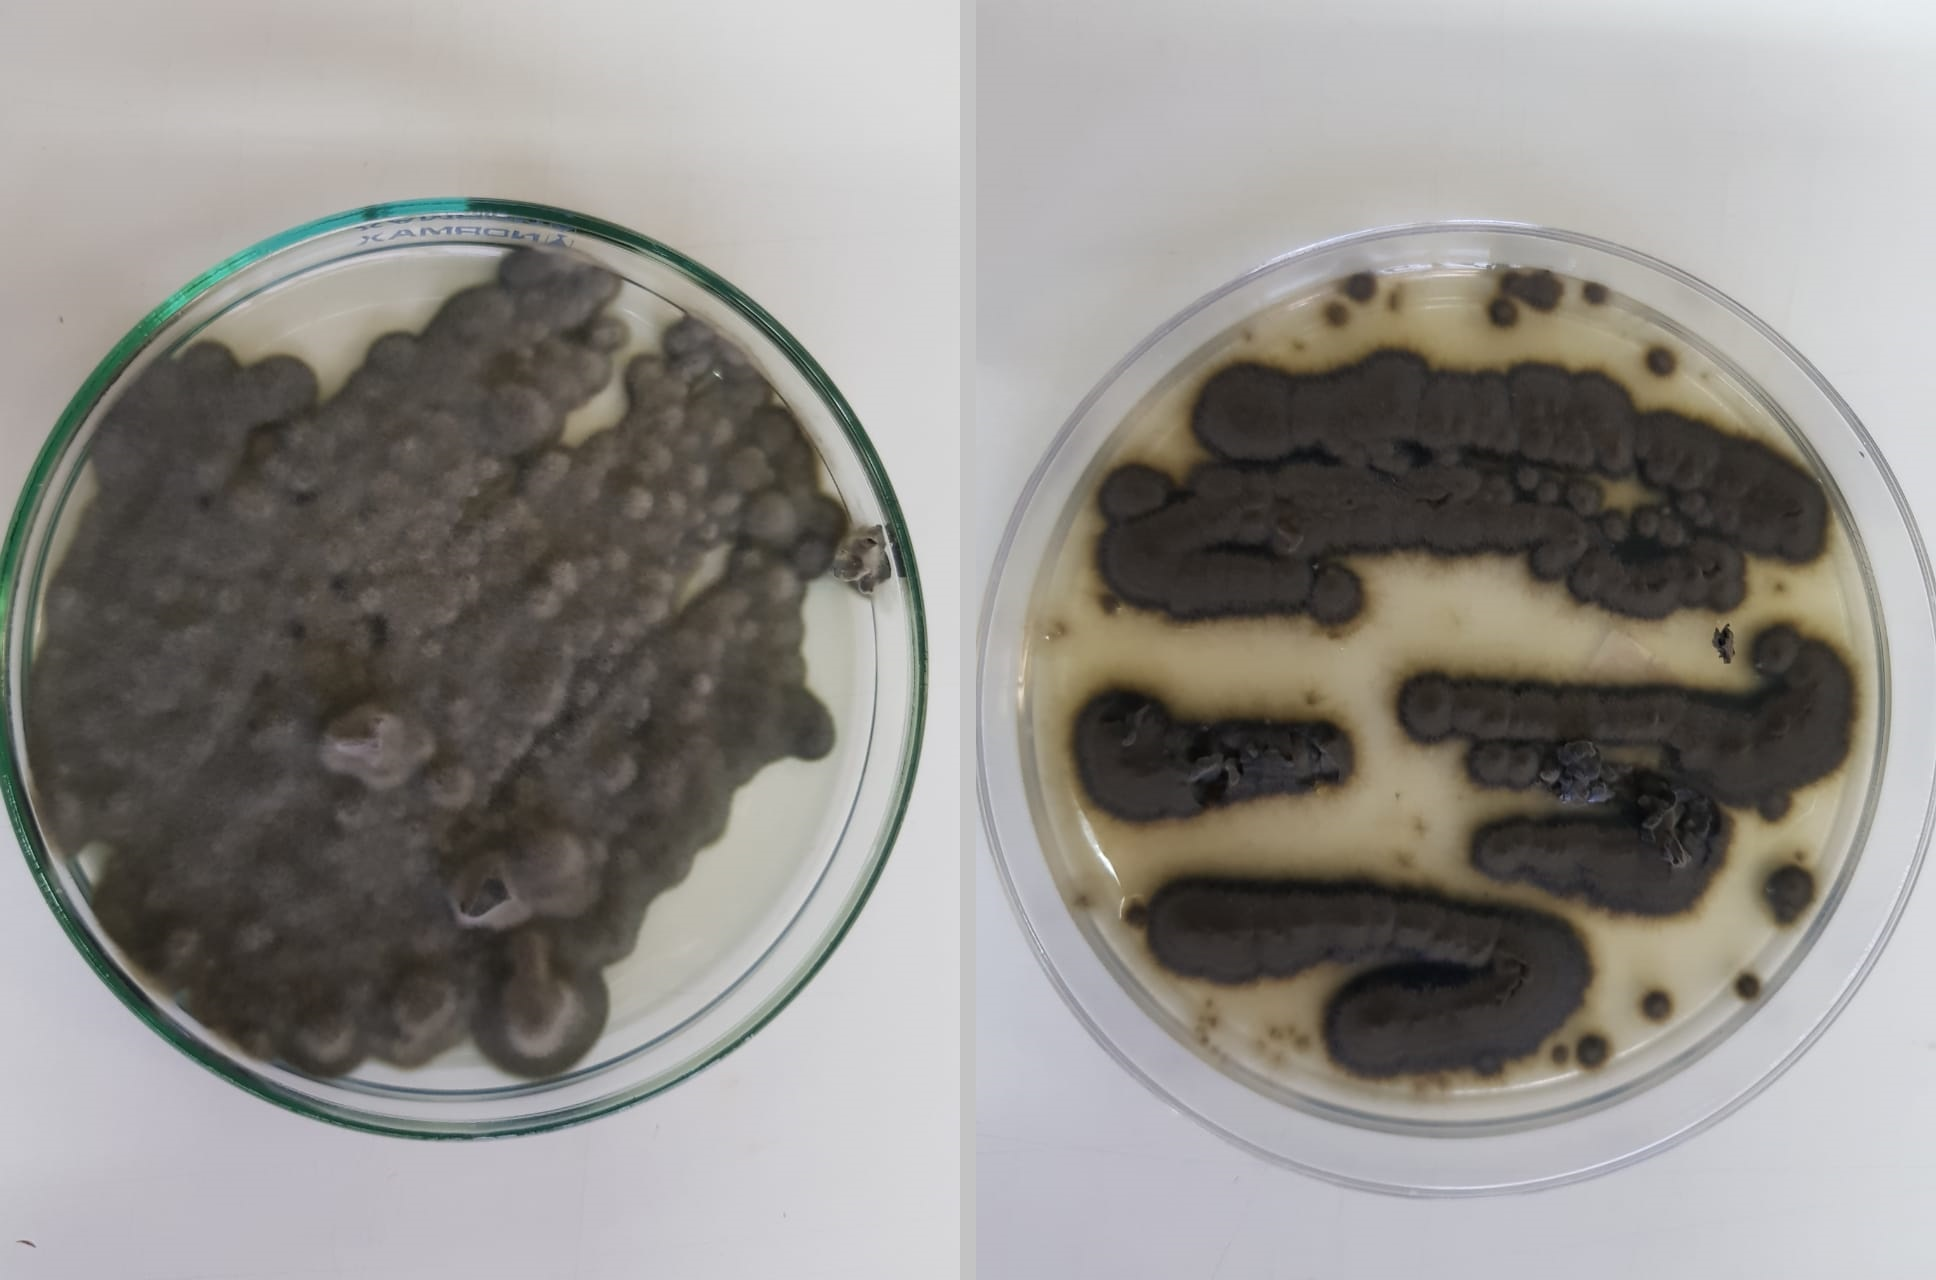
\includegraphics[width=6cm]{pedrosoi_pugnacius}
\caption{Fungo Fonsecaea pedrosoi e Fonsecaea pugnacius respectivamente. Fonte: Pesquisadora Juliana Thaler}
\label{pedrosoi_pugnacius}
\end{figure}

Para cada gênero de fungo as amostras serão submetidas a uma correção de linha base e a uma normalização e então submetidas ao PCA para que apenas as informações mais relevantes do espectro sirvam como dados de entrada para a rede neural artificial a ser criada e treinada. A quantidade de componentes escolhidas será feita mediante análise da variância das mesmas, bem como, das plotagens de comparação entre as componentes. Para o treinamento da rede neural artificial serão utilizados 80\% dos dados disponíveis e os outros 20\% serão utilizados na validação da efetividade da mesma.

\section{Discussão e resultados esperados}

A escolha de aplicar a rede neural artificial apenas as componentes de maior relevância do espectro Raman é feita com o propósito de eliminar ruídos que possam estar contidos nas amostras avaliadas. \cite{Butler2016} cita o PCA como uma poderosa ferramenta na eliminação de ruídos e reconstrução do espectro Raman apenas com as principais componentes. \cite{DeGoes2016} conclui em seu experimento que quando não é possível visualizar agrupamentos de forma clara apenas utilizando-se de PCA, treinar as redes neurais artificiais com os resultados do PCA pode aprimorar a classificação das amostras.

Para que o PCA exerça sua função da forma esperada, são necessários aplicar dois procedimentos as amostras: correção de linha base e normalização. A correção de linha base é necessária, por conta do mascaramento do sinal relevante que o espectro Raman sofre em virtude da fluorescência \cite{DeGoes2016}, fenômeno o qual a Espectroscopia Raman está sujeita. A normalização, por sua vez, deve ocorrer porque as amostras podem ter sido obtidas sobre diferentes calibrações dos aparelhos de microscopia, gerando diferentes intervalos nas frequências amostradas. Na Figura \ref{baseline_correction_normalization} está demonstrado um exemplo gráfico da correção de linha base e normalização.

\begin{figure}[ht]
\centering
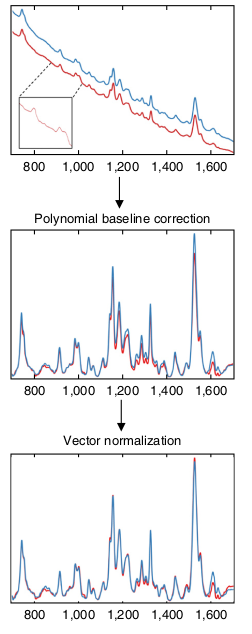
\includegraphics[width=6cm]{baseline_correction_normalization}
\caption{Gráfico da transformação da assinatura do espectro Raman após as operações de correção de linha base e normalização. Fonte: \cite{Butler2016}}
\label{baseline_correction_normalization}
\end{figure}

Quanto a arquitetura da rede neural artificial, diferentes configurações podem ser experimentadas de forma a identificar qual atinge o melhor resultado consumindo o menor quantidade de recursos computacionais.

Ao fim dessa pesquisa espera-se obter duas redes neurais artificiais treinadas capazes de a partir do dados do espectro Raman de um fungo identificar a qual espécie ele pertence. Contudo, elas não serão genéricas, elas serão aptas a distinguir espécies entre gêneros iguais. Então a primeira rede neural artificial será capaz de distiguir espécies de fungos do gênero Candida e a segunda distinguir espécies do gênero Fonsecaea. 

\section{Conclusão}
 
A relevância deste trabalho dar-se-á pela possibilidade criar um método de identificação de espécies de fungos mais simples do que o sequenciamento genético.

\section*{Reconhecimento}

Ao Professor Hugo Vieria Neto, Ph.D. pelas aulas ministradas na displina de Metodologia Científica do programa de pós graduação da Universidade Tecnológica Federal do Paraná.

\bibliographystyle{IEEEtran}
\bibliography{IEEEabrv,modref}

\end{document}